% LaTeX test file for lexer testing
\documentclass[12pt,a4paper]{article}

% Package imports
\usepackage[utf8]{inputenc}
\usepackage[T1]{fontenc}
\usepackage[english]{babel}
\usepackage{amsmath}
\usepackage{amsfonts}
\usepackage{amssymb}
\usepackage{amsthm}
\usepackage{graphicx}
\usepackage{color}
\usepackage{xcolor}
\usepackage{hyperref}
\usepackage{geometry}
\usepackage{fancyhdr}
\usepackage{listings}
\usepackage{tikz}
\usepackage{pgfplots}
\usepackage{booktabs}
\usepackage{array}
\usepackage{longtable}
\usepackage{multirow}
\usepackage{multicol}
\usepackage{enumerate}
\usepackage{enumitem}
\usepackage{float}
\usepackage{caption}
\usepackage{subcaption}
\usepackage{algorithm}
\usepackage{algorithmic}
\usepackage{verbatim}
\usepackage{url}
\usepackage{natbib}

% Page geometry
\geometry{
    left=2.5cm,
    right=2.5cm,
    top=3cm,
    bottom=3cm
}

% Header and footer
\pagestyle{fancy}
\fancyhf{}
\fancyhead[L]{\leftmark}
\fancyhead[R]{\thepage}
\fancyfoot[C]{LaTeX Test Document}

% Custom colors
\definecolor{codegreen}{rgb}{0,0.6,0}
\definecolor{codegray}{rgb}{0.5,0.5,0.5}
\definecolor{codepurple}{rgb}{0.58,0,0.82}
\definecolor{backcolour}{rgb}{0.95,0.95,0.92}

% Code listing style
\lstdefinestyle{mystyle}{
    backgroundcolor=\color{backcolour},   
    commentstyle=\color{codegreen},
    keywordstyle=\color{magenta},
    numberstyle=\tiny\color{codegray},
    stringstyle=\color{codepurple},
    basicstyle=\ttfamily\footnotesize,
    breakatwhitespace=false,         
    breaklines=true,                 
    captionpos=b,                    
    keepspaces=true,                 
    numbers=left,                    
    numbersep=5pt,                  
    showspaces=false,                
    showstringspaces=false,
    showtabs=false,                  
    tabsize=2
}

\lstset{style=mystyle}

% Custom commands
\newcommand{\R}{\mathbb{R}}
\newcommand{\N}{\mathbb{N}}
\newcommand{\Z}{\mathbb{Z}}
\newcommand{\Q}{\mathbb{Q}}
\newcommand{\C}{\mathbb{C}}
\newcommand{\norm}[1]{\left\lVert#1\right\rVert}
\newcommand{\abs}[1]{\left|#1\right|}
\newcommand{\set}[1]{\left\{#1\right\}}
\newcommand{\seq}[1]{\left\langle#1\right\rangle}
\newcommand{\eps}{\varepsilon}
\newcommand{\To}{\longrightarrow}
\newcommand{\BX}{\mathbf{B}(X)}
\newcommand{\A}{\mathcal{A}}

% Theorem environments
\newtheorem{theorem}{Theorem}[section]
\newtheorem{lemma}[theorem]{Lemma}
\newtheorem{proposition}[theorem]{Proposition}
\newtheorem{corollary}[theorem]{Corollary}
\newtheorem{definition}[theorem]{Definition}
\newtheorem{example}[theorem]{Example}
\newtheorem{remark}[theorem]{Remark}

% Document metadata
\title{Comprehensive \LaTeX{} Test Document}
\author{Test Author\\
        Department of Computer Science\\
        University of Testing\\
        \texttt{test@example.com}}
\date{\today}

% TikZ libraries
\usetikzlibrary{arrows,shapes,positioning,shadows,trees}

\begin{document}

\maketitle

\begin{abstract}
This document serves as a comprehensive test for \LaTeX{} lexer functionality. It includes various mathematical expressions, formatting commands, environments, and advanced features commonly used in academic and technical documents. The purpose is to ensure proper parsing and highlighting of \LaTeX{} syntax elements.
\end{abstract}

\tableofcontents
\newpage

\section{Introduction}

This is a test document for \LaTeX{} lexer testing. It contains various \LaTeX{} constructs including:
\begin{itemize}
    \item Mathematical expressions and equations
    \item Tables and figures
    \item Lists and enumerations
    \item Cross-references and citations
    \item Custom commands and environments
    \item Code listings
    \item TikZ graphics
\end{itemize}

\section{Text Formatting}

\subsection{Basic Formatting}

This is \textbf{bold text}, this is \textit{italic text}, and this is \texttt{typewriter text}. We can also use \emph{emphasized text} and \underline{underlined text}.

\subsection{Font Sizes}

{\tiny This is tiny text.}
{\scriptsize This is script size text.}
{\footnotesize This is footnote size text.}
{\small This is small text.}
{\normalsize This is normal size text.}
{\large This is large text.}
{\Large This is Large text.}
{\LARGE This is LARGE text.}
{\huge This is huge text.}
{\Huge This is Huge text.}

\subsection{Colors}

This text is in \textcolor{red}{red}, this is in \textcolor{blue}{blue}, and this is in \textcolor{green}{green}.

\colorbox{yellow}{This text has a yellow background.}

\section{Mathematical Expressions}

\subsection{Inline Mathematics}

The quadratic formula is $x = \frac{-b \pm \sqrt{b^2 - 4ac}}{2a}$. The area of a circle is $A = \pi r^2$. Euler's identity states that $e^{i\pi} + 1 = 0$.

\subsection{Display Mathematics}

The fundamental theorem of calculus:
\begin{equation}
\int_a^b f'(x) \, dx = f(b) - f(a)
\end{equation}

The Taylor series expansion:
\begin{equation}
f(x) = \sum_{n=0}^{\infty} \frac{f^{(n)}(a)}{n!}(x-a)^n
\end{equation}

\subsection{Aligned Equations}

\begin{align}
\nabla \cdot \mathbf{E} &= \frac{\rho}{\epsilon_0} \\
\nabla \cdot \mathbf{B} &= 0 \\
\nabla \times \mathbf{E} &= -\frac{\partial \mathbf{B}}{\partial t} \\
\nabla \times \mathbf{B} &= \mu_0\mathbf{J} + \mu_0\epsilon_0\frac{\partial \mathbf{E}}{\partial t}
\end{align}

\subsection{Matrices}

\begin{equation}
\mathbf{A} = \begin{pmatrix}
a_{11} & a_{12} & \cdots & a_{1n} \\
a_{21} & a_{22} & \cdots & a_{2n} \\
\vdots & \vdots & \ddots & \vdots \\
a_{m1} & a_{m2} & \cdots & a_{mn}
\end{pmatrix}
\end{equation}

\begin{equation}
\det(\mathbf{A}) = \begin{vmatrix}
a & b \\
c & d
\end{vmatrix} = ad - bc
\end{equation}

\subsection{Complex Mathematical Expressions}

\begin{equation}
\oint_{\partial D} \mathbf{F} \cdot d\mathbf{r} = \iint_D \left(\frac{\partial Q}{\partial x} - \frac{\partial P}{\partial y}\right) dx \, dy
\end{equation}

\begin{equation}
\lim_{n \to \infty} \left(1 + \frac{1}{n}\right)^n = e
\end{equation}

\begin{equation}
\sum_{n=1}^{\infty} \frac{1}{n^2} = \frac{\pi^2}{6}
\end{equation}

\section{Theorem Environments}

\begin{definition}
A \emph{metric space} is a set $X$ together with a function $d: X \times X \to \R$ such that for all $x, y, z \in X$:
\begin{enumerate}
    \item $d(x, y) \geq 0$ and $d(x, y) = 0$ if and only if $x = y$
    \item $d(x, y) = d(y, x)$
    \item $d(x, z) \leq d(x, y) + d(y, z)$
\end{enumerate}
\end{definition}

\begin{theorem}[Pythagorean Theorem]
In a right triangle with legs of length $a$ and $b$ and hypotenuse of length $c$, we have
\begin{equation}
a^2 + b^2 = c^2
\end{equation}
\end{theorem}

\begin{proof}
This is a classic proof by geometric construction...
\end{proof}

\begin{lemma}
Every convergent sequence is bounded.
\end{lemma}

\begin{corollary}
Every convergent sequence is Cauchy.
\end{corollary}

\section{Lists and Enumerations}

\subsection{Itemized Lists}

\begin{itemize}
    \item First item
    \item Second item
        \begin{itemize}
            \item Nested item 1
            \item Nested item 2
        \end{itemize}
    \item Third item
\end{itemize}

\subsection{Enumerated Lists}

\begin{enumerate}
    \item First numbered item
    \item Second numbered item
        \begin{enumerate}
            \item Nested numbered item 1
            \item Nested numbered item 2
        \end{enumerate}
    \item Third numbered item
\end{enumerate}

\subsection{Custom Enumerations}

\begin{enumerate}[label=(\alph*)]
    \item Item a
    \item Item b
    \item Item c
\end{enumerate}

\begin{enumerate}[label=\Roman*.]
    \item Item I
    \item Item II
    \item Item III
\end{enumerate}

\section{Tables}

\subsection{Basic Table}

\begin{table}[H]
\centering
\caption{Sample Data Table}
\label{tab:sample}
\begin{tabular}{|c|c|c|}
\hline
\textbf{Name} & \textbf{Age} & \textbf{Score} \\
\hline
Alice & 25 & 95 \\
Bob & 30 & 87 \\
Charlie & 22 & 92 \\
\hline
\end{tabular}
\end{table}

\subsection{Advanced Table}

\begin{table}[H]
\centering
\caption{Advanced Table with Multiple Features}
\label{tab:advanced}
\begin{tabular}{@{}lccr@{}}
\toprule
\textbf{Item} & \textbf{Quantity} & \textbf{Price (\$)} & \textbf{Total (\$)} \\
\midrule
Apples & 10 & 0.50 & 5.00 \\
Bananas & 6 & 0.30 & 1.80 \\
Oranges & 8 & 0.75 & 6.00 \\
\midrule
\multicolumn{3}{r}{\textbf{Grand Total:}} & \textbf{12.80} \\
\bottomrule
\end{tabular}
\end{table}

\section{Figures and Graphics}

\subsection{Simple Figure}

\begin{figure}[H]
\centering
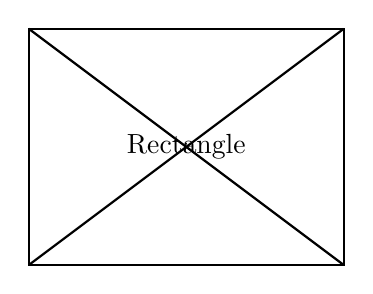
\begin{tikzpicture}
\draw[thick] (0,0) -- (4,0) -- (4,3) -- (0,3) -- cycle;
\draw[thick] (0,0) -- (4,3);
\draw[thick] (0,3) -- (4,0);
\node at (2,1.5) {Rectangle};
\end{tikzpicture}
\caption{A simple rectangle with diagonals}
\label{fig:rectangle}
\end{figure}

\subsection{Mathematical Plot}

\begin{figure}[H]
\centering
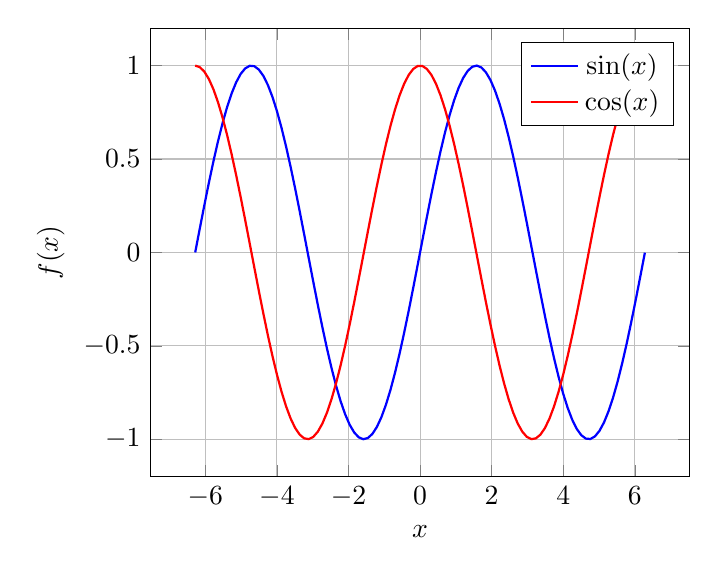
\begin{tikzpicture}
\begin{axis}[
    xlabel={$x$},
    ylabel={$f(x)$},
    domain=-2*pi:2*pi,
    samples=100,
    grid=major,
    legend pos=north east
]
\addplot[blue, thick] {sin(deg(x))};
\addplot[red, thick] {cos(deg(x))};
\legend{$\sin(x)$, $\cos(x)$}
\end{axis}
\end{tikzpicture}
\caption{Sine and cosine functions}
\label{fig:trigfunctions}
\end{figure}

\section{Code Listings}

\subsection{Python Code}

\begin{lstlisting}[language=Python, caption=Python Example]
def fibonacci(n):
    """Calculate the nth Fibonacci number."""
    if n <= 1:
        return n
    else:
        return fibonacci(n-1) + fibonacci(n-2)

# Test the function
for i in range(10):
    print(f"F({i}) = {fibonacci(i)}")
\end{lstlisting}

\subsection{C++ Code}

\begin{lstlisting}[language=C++, caption=C++ Example]
#include <iostream>
#include <vector>

class Matrix {
private:
    std::vector<std::vector<double>> data;
    int rows, cols;

public:
    Matrix(int r, int c) : rows(r), cols(c) {
        data.resize(rows, std::vector<double>(cols, 0.0));
    }
    
    double& operator()(int i, int j) {
        return data[i][j];
    }
    
    void print() {
        for (int i = 0; i < rows; ++i) {
            for (int j = 0; j < cols; ++j) {
                std::cout << data[i][j] << " ";
            }
            std::cout << std::endl;
        }
    }
};
\end{lstlisting}

\section{Algorithms}

\begin{algorithm}
\caption{Quicksort Algorithm}
\label{alg:quicksort}
\begin{algorithmic}[1]
\REQUIRE Array $A[1..n]$ of comparable elements
\ENSURE Array $A$ sorted in non-decreasing order
\PROCEDURE{QuickSort}{$A, p, r$}
    \IF{$p < r$}
        \STATE $q \leftarrow$ \CALL{Partition}{$A, p, r$}
        \STATE \CALL{QuickSort}{$A, p, q-1$}
        \STATE \CALL{QuickSort}{$A, q+1, r$}
    \ENDIF
\ENDPROCEDURE
\PROCEDURE{Partition}{$A, p, r$}
    \STATE $x \leftarrow A[r]$
    \STATE $i \leftarrow p - 1$
    \FOR{$j \leftarrow p$ \TO $r-1$}
        \IF{$A[j] \leq x$}
            \STATE $i \leftarrow i + 1$
            \STATE exchange $A[i]$ with $A[j]$
        \ENDIF
    \ENDFOR
    \STATE exchange $A[i+1]$ with $A[r]$
    \RETURN $i+1$
\ENDPROCEDURE
\end{algorithmic}
\end{algorithm}

\section{Cross-References and Citations}

As we can see in Table~\ref{tab:sample}, the data shows interesting patterns. Figure~\ref{fig:rectangle} illustrates a geometric construction, while Figure~\ref{fig:trigfunctions} shows mathematical functions.

The algorithm described in Algorithm~\ref{alg:quicksort} has a time complexity of $O(n \log n)$ on average.

According to \cite{knuth1997art}, the analysis of algorithms is fundamental to computer science. The work by \cite{cormen2009introduction} provides comprehensive coverage of algorithmic techniques.

\section{Special Characters and Symbols}

\subsection{Greek Letters}

$\alpha, \beta, \gamma, \delta, \epsilon, \zeta, \eta, \theta, \iota, \kappa, \lambda, \mu, \nu, \xi, \omicron, \pi, \rho, \sigma, \tau, \upsilon, \phi, \chi, \psi, \omega$

$\Alpha, \Beta, \Gamma, \Delta, \Epsilon, \Zeta, \Eta, \Theta, \Iota, \Kappa, \Lambda, \Mu, \Nu, \Xi, \Omicron, \Pi, \Rho, \Sigma, \Tau, \Upsilon, \Phi, \Chi, \Psi, \Omega$

\subsection{Mathematical Symbols}

$\infty, \partial, \nabla, \sum, \prod, \int, \oint, \pm, \mp, \times, \div, \cdot, \ast, \star, \circ, \bullet, \cap, \cup, \subset, \supset, \subseteq, \supseteq, \in, \notin, \emptyset, \forall, \exists, \neg, \land, \lor, \implies, \iff$

\subsection{Arrows}

$\leftarrow, \rightarrow, \leftrightarrow, \Leftarrow, \Rightarrow, \Leftrightarrow, \uparrow, \downarrow, \updownarrow, \nearrow, \searrow, \swarrow, \nwarrow$

\section{Verbatim Text}

\begin{verbatim}
This is verbatim text.
It preserves    spacing   and
special characters like $ % & # _ { } \ ^ ~
No LaTeX commands are processed here.
\end{verbatim}

\section{Multiple Columns}

\begin{multicols}{2}
This text is typeset in two columns. Lorem ipsum dolor sit amet, consectetur adipiscing elit. Sed do eiusmod tempor incididunt ut labore et dolore magna aliqua. Ut enim ad minim veniam, quis nostrud exercitation ullamco laboris nisi ut aliquip ex ea commodo consequat.

Duis aute irure dolor in reprehenderit in voluptate velit esse cillum dolore eu fugiat nulla pariatur. Excepteur sint occaecat cupidatat non proident, sunt in culpa qui officia deserunt mollit anim id est laborum.

Sed ut perspiciatis unde omnis iste natus error sit voluptatem accusantium doloremque laudantium, totam rem aperiam, eaque ipsa quae ab illo inventore veritatis et quasi architecto beatae vitae dicta sunt explicabo.
\end{multicols}

\section{Footnotes and Marginal Notes}

This text has a footnote\footnote{This is a footnote explaining something important.}. Here's another sentence with a footnote\footnote{Another footnote with additional information.}.

\marginpar{This is a marginal note that appears in the margin.}

\section{Hyperlinks and URLs}

Visit \url{https://www.latex-project.org/} for more information about \LaTeX{}. You can also check out \href{https://www.overleaf.com/}{Overleaf} for online \LaTeX{} editing.

\section{Custom Environments}

\newenvironment{myquote}
{\begin{quote}\itshape}
{\end{quote}}

\begin{myquote}
This is a custom quote environment that makes text italic and indented.
\end{myquote}

\section{Conclusion}

This document demonstrates various \LaTeX{} features and constructs that should be properly handled by a lexer. It includes mathematical expressions, formatting commands, environments, cross-references, and many other elements commonly found in \LaTeX{} documents.

% Bibliography
\begin{thebibliography}{99}

\bibitem{knuth1997art}
Knuth, D. E. (1997).
\emph{The Art of Computer Programming, Volume 1: Fundamental Algorithms}.
Addison-Wesley Professional, 3rd edition.

\bibitem{cormen2009introduction}
Cormen, T. H., Leiserson, C. E., Rivest, R. L., and Stein, C. (2009).
\emph{Introduction to Algorithms}.
MIT Press, 3rd edition.

\bibitem{lamport1994latex}
Lamport, L. (1994).
\emph{\LaTeX{}: A Document Preparation System}.
Addison-Wesley Professional, 2nd edition.

\end{thebibliography}

\appendix

\section{Additional Mathematical Formulas}

\subsection{Calculus}

\begin{align}
\frac{d}{dx}[x^n] &= nx^{n-1} \\
\frac{d}{dx}[e^x] &= e^x \\
\frac{d}{dx}[\ln x] &= \frac{1}{x} \\
\frac{d}{dx}[\sin x] &= \cos x \\
\frac{d}{dx}[\cos x] &= -\sin x
\end{align}

\subsection{Linear Algebra}

\begin{equation}
\mathbf{A}\mathbf{x} = \mathbf{b}
\end{equation}

\begin{equation}
\mathbf{A}^{-1} = \frac{1}{\det(\mathbf{A})} \text{adj}(\mathbf{A})
\end{equation}

\subsection{Statistics}

\begin{equation}
\bar{x} = \frac{1}{n}\sum_{i=1}^{n} x_i
\end{equation}

\begin{equation}
s^2 = \frac{1}{n-1}\sum_{i=1}^{n} (x_i - \bar{x})^2
\end{equation}

\begin{equation}
P(A|B) = \frac{P(B|A)P(A)}{P(B)}
\end{equation}

\end{document}